\chapter{Résultats sur corps humain complet}
\label{annexe:kyoto}


Dans cette annexe nous présentons les résultats de la simulation
présentée dans la section \ref{ssect:corps_complet}.
Cette simulation met en scène un modèle de corps humain complet
(comprenant $12$ organes, le squelette et la peau)
avec une antenne de technologie LTCC placée entre le bras
gauche et le corps.
Le temps physique simulé est de $10$ ns.
Nous présentons les résultats en plan de coupe à
chaque nanoseconde écoulée.

\begin{figure}[!h]
	\centering
	\caption{
		\label{img:annexe_kyoto_cutplane_1ns}
		Résultats en plan de coupe $(\x_1 O \x_3)$
		en $\x_2 = -0.1255$ m (antenne)
		au temps $t=1$ ns.
	}
	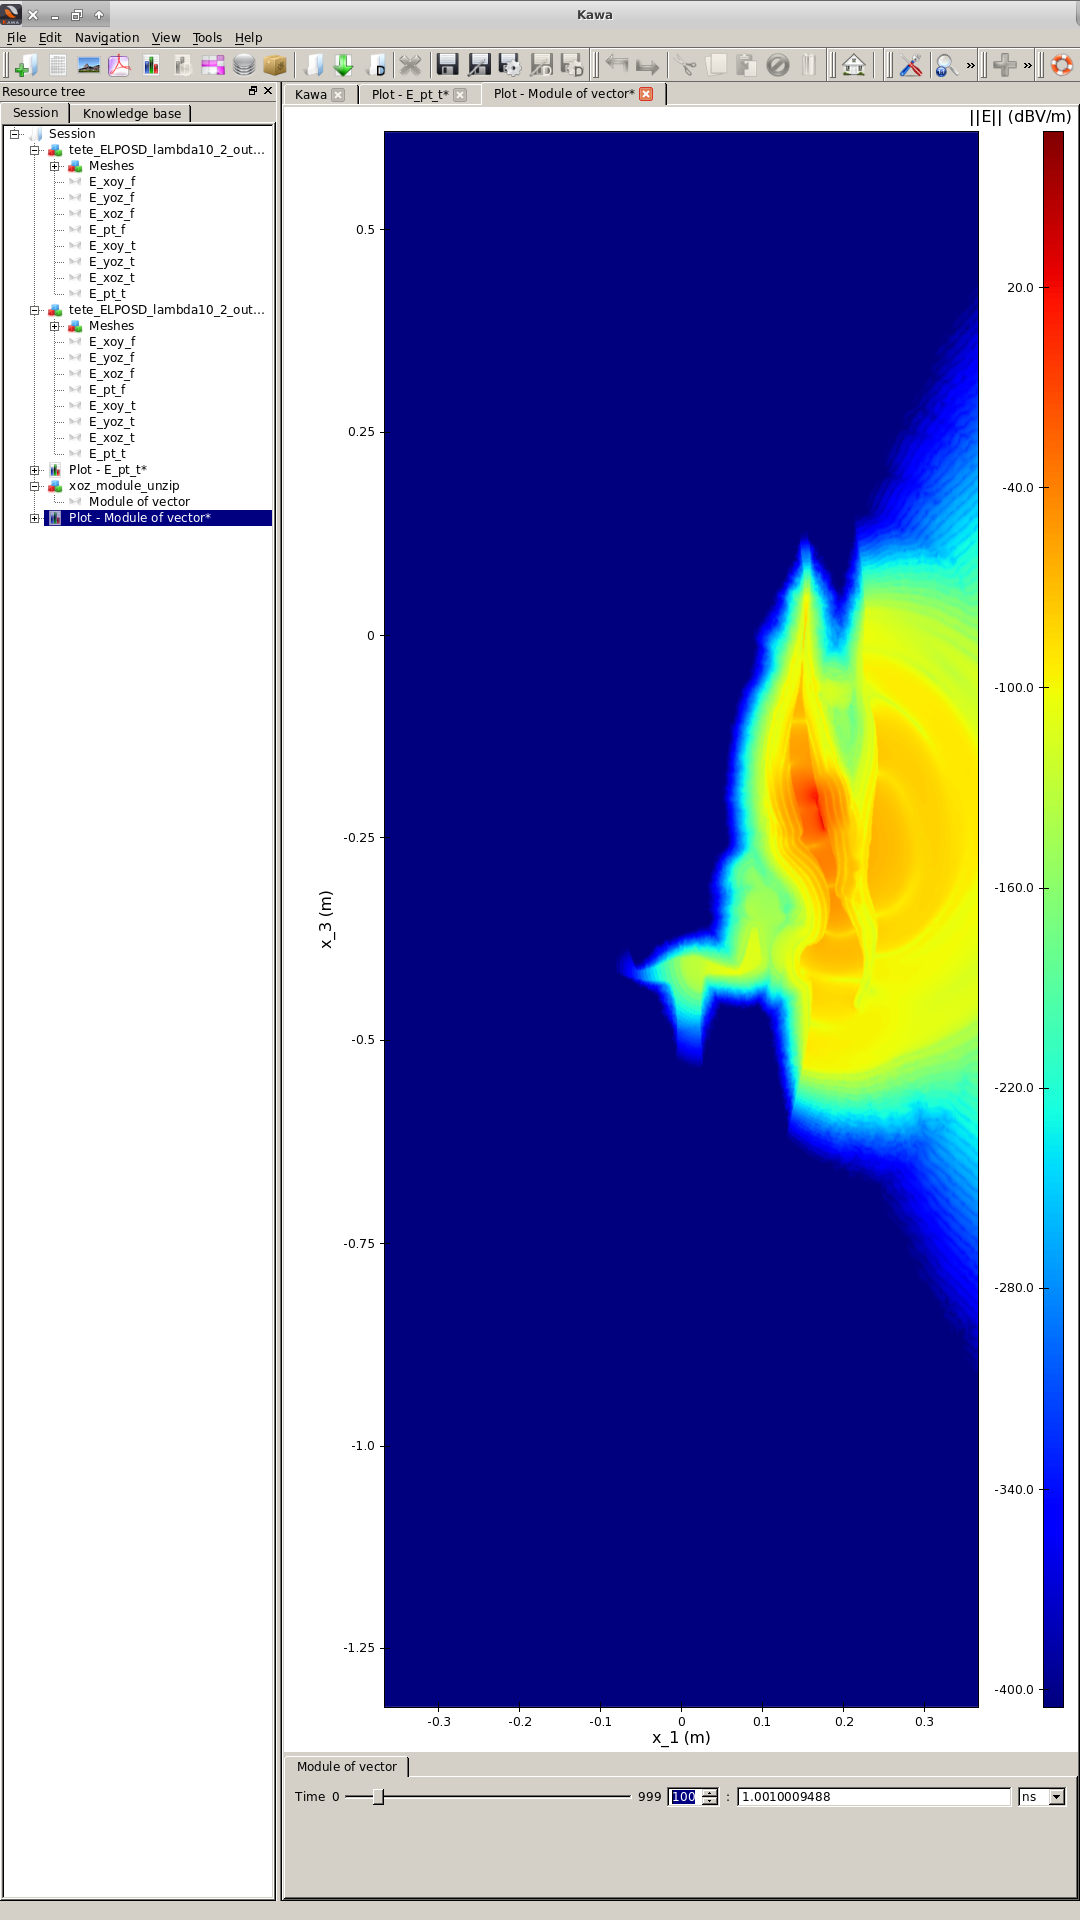
\includegraphics[
		width=0.66\linewidth,
		trim={317 170 8 108},clip
	]{kyoto_1ns}
\end{figure}

\begin{figure}[!h]
	\centering
	\caption{
		\label{img:annexe_kyoto_cutplane_2ns}
		Résultats en plan de coupe $(\x_1 O \x_3)$
		en $\x_2 = -0.1255$ m (antenne)
		au temps $t=2$ ns.
	}
	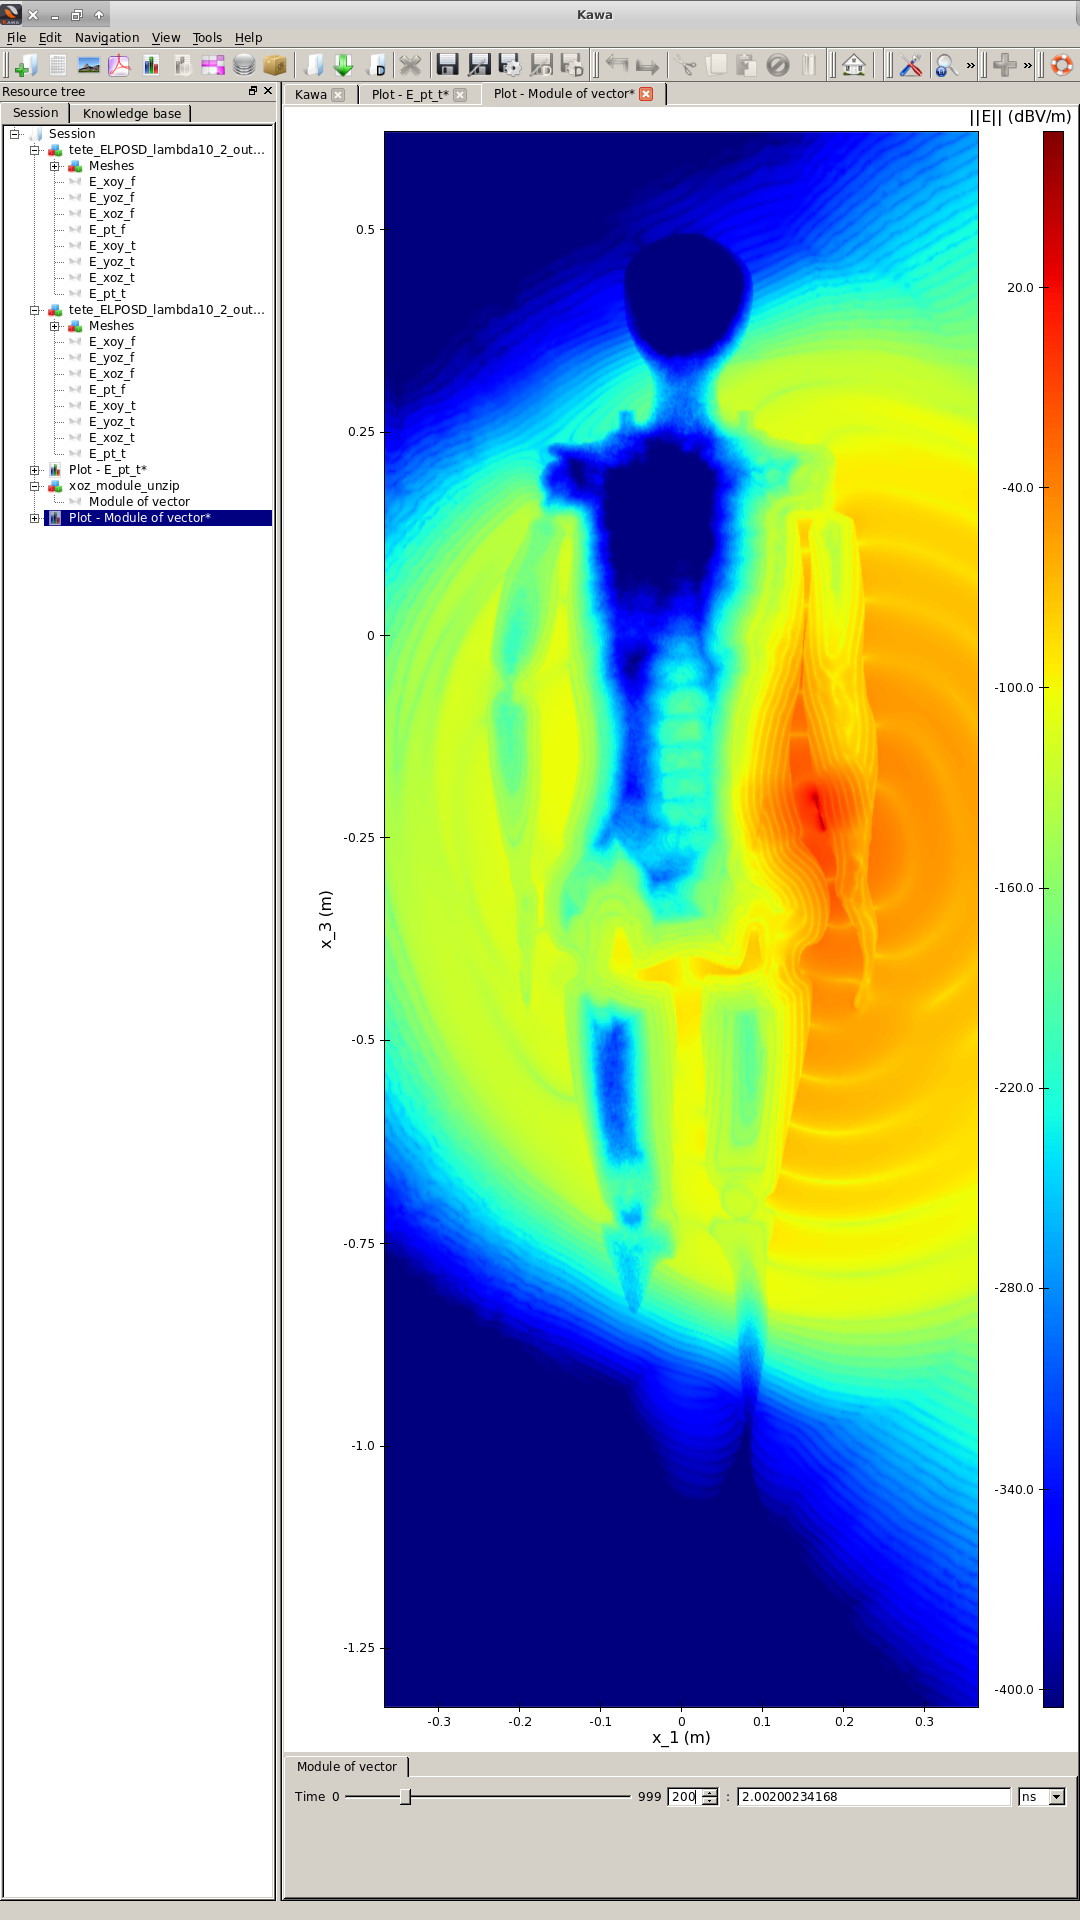
\includegraphics[
		width=0.66\linewidth,
		trim={317 170 8 108},clip
	]{kyoto_2ns}
\end{figure}

\begin{figure}[!h]
	\centering
	\caption{
		\label{img:annexe_kyoto_cutplane_3ns}
		Résultats en plan de coupe $(\x_1 O \x_3)$
		en $\x_2 = -0.1255$ m (antenne)
		au temps $t=3$ ns.
	}
	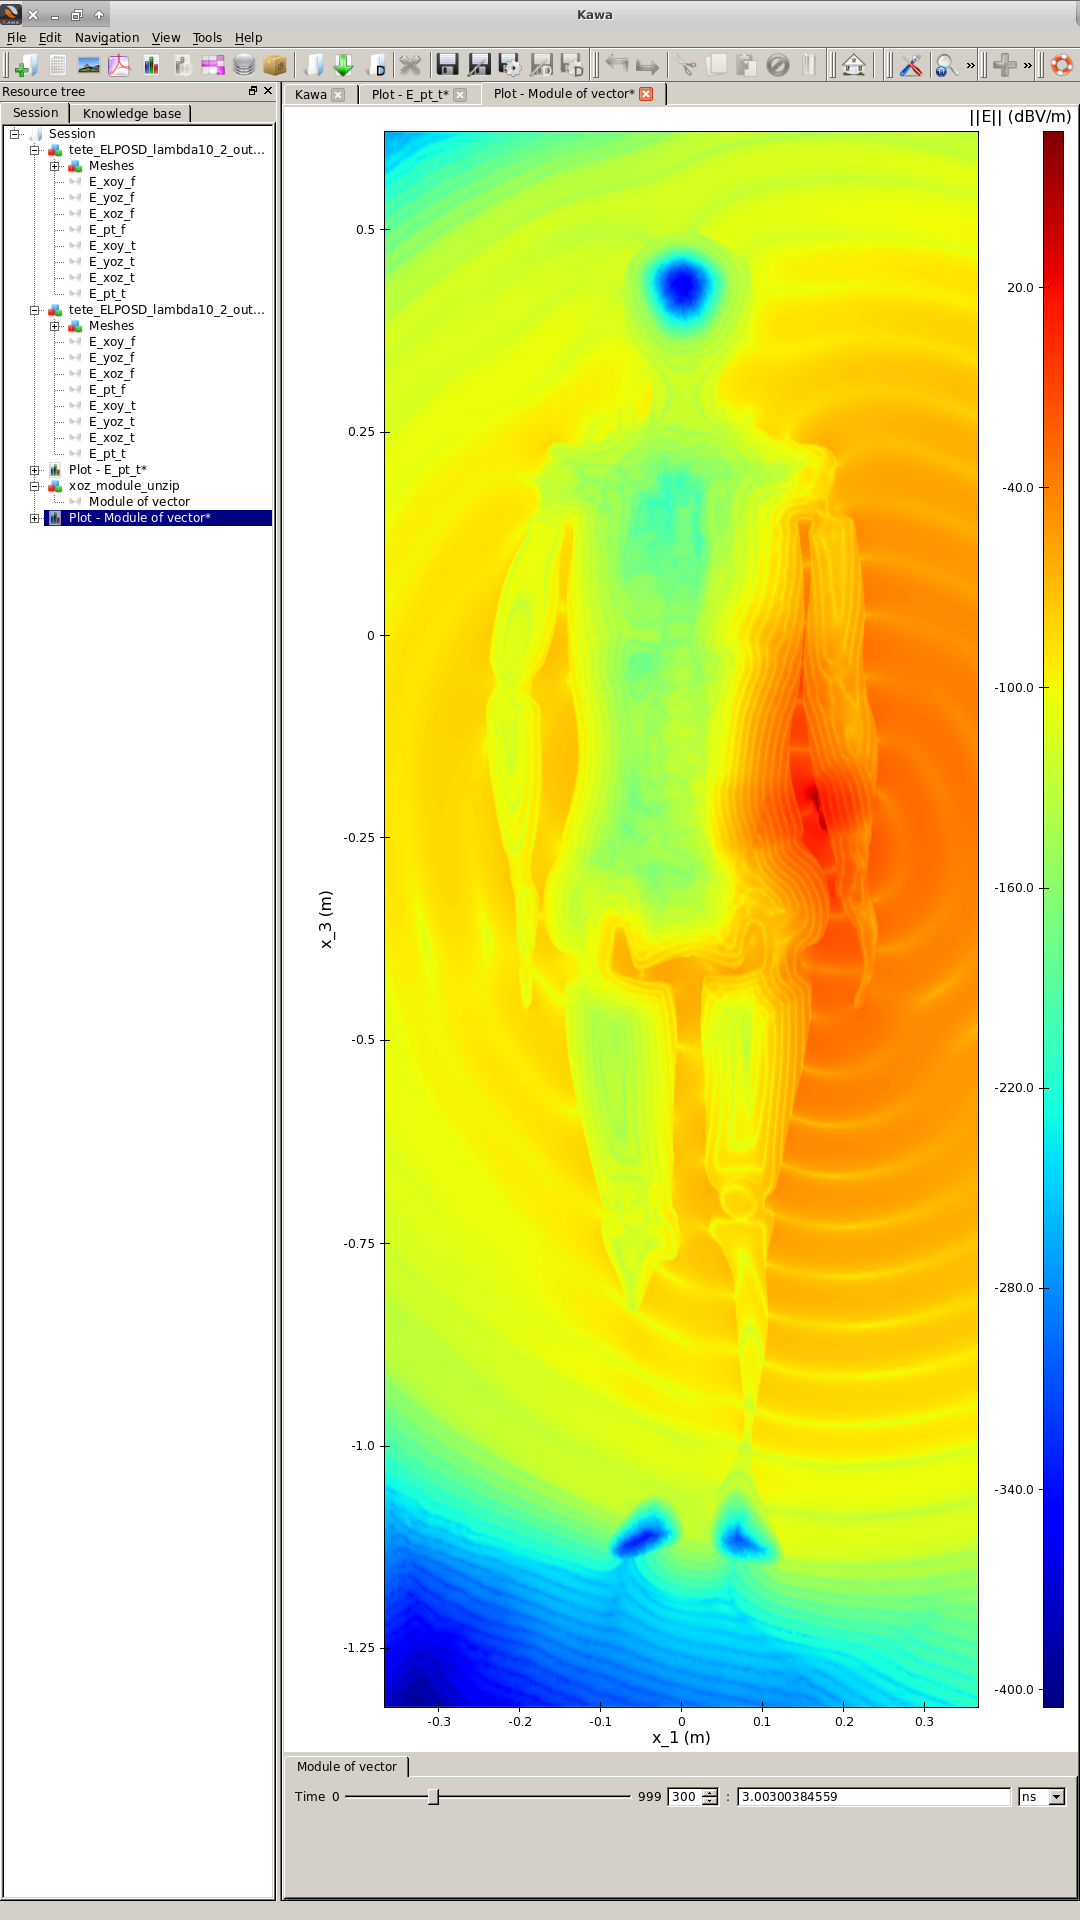
\includegraphics[
	width=0.66\linewidth,
	trim={317 170 8 108},clip
	]{kyoto_3ns}
\end{figure}

\begin{figure}[!h]
	\centering
	\caption{
		\label{img:annexe_kyoto_cutplane_4ns}
		Résultats en plan de coupe $(\x_1 O \x_3)$
		en $\x_2 = -0.1255$ m (antenne)
		au temps $t=4$ ns.
	}
	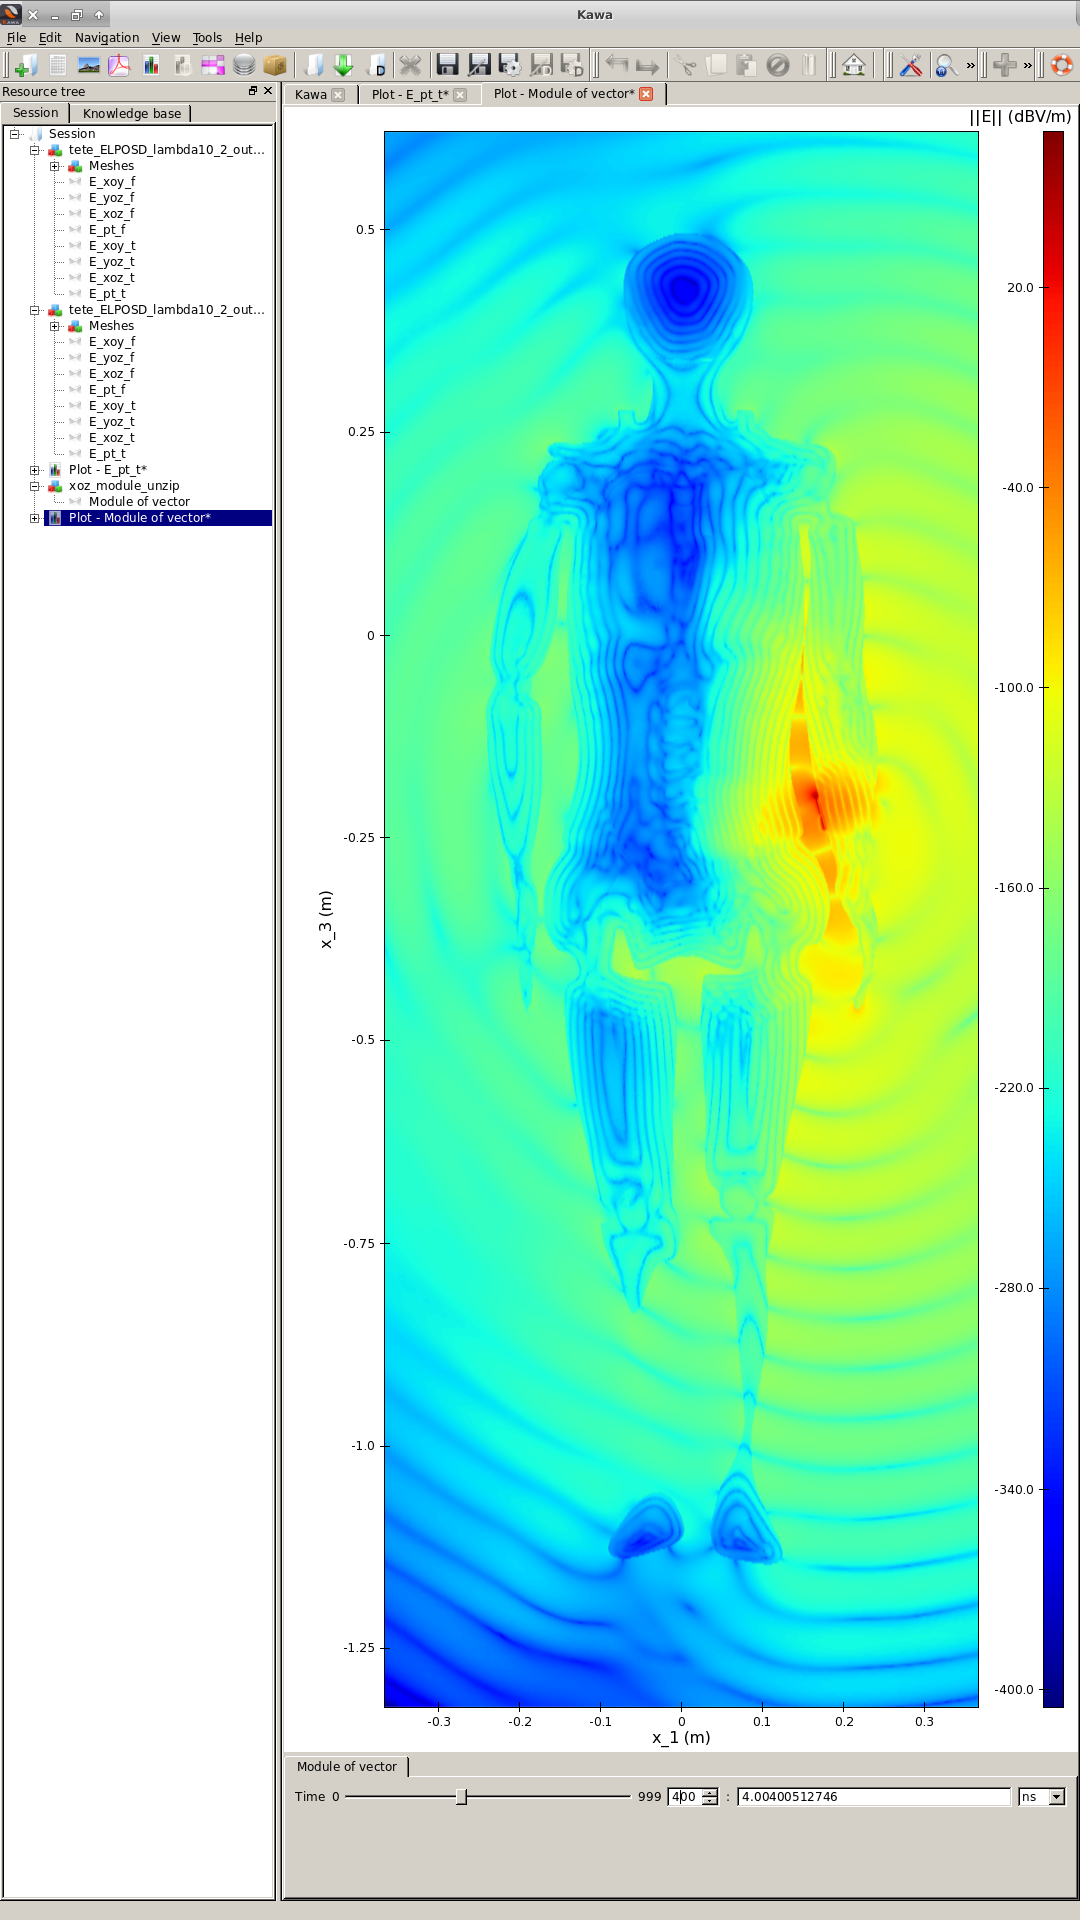
\includegraphics[
	width=0.66\linewidth,
	trim={317 170 8 108},clip
	]{kyoto_4ns}
\end{figure}

\begin{figure}[!h]
	\centering
	\caption{
		\label{img:annexe_kyoto_cutplane_5ns}
		Résultats en plan de coupe $(\x_1 O \x_3)$
		en $\x_2 = -0.1255$ m (antenne)
		au temps $t=5$ ns.
	}
	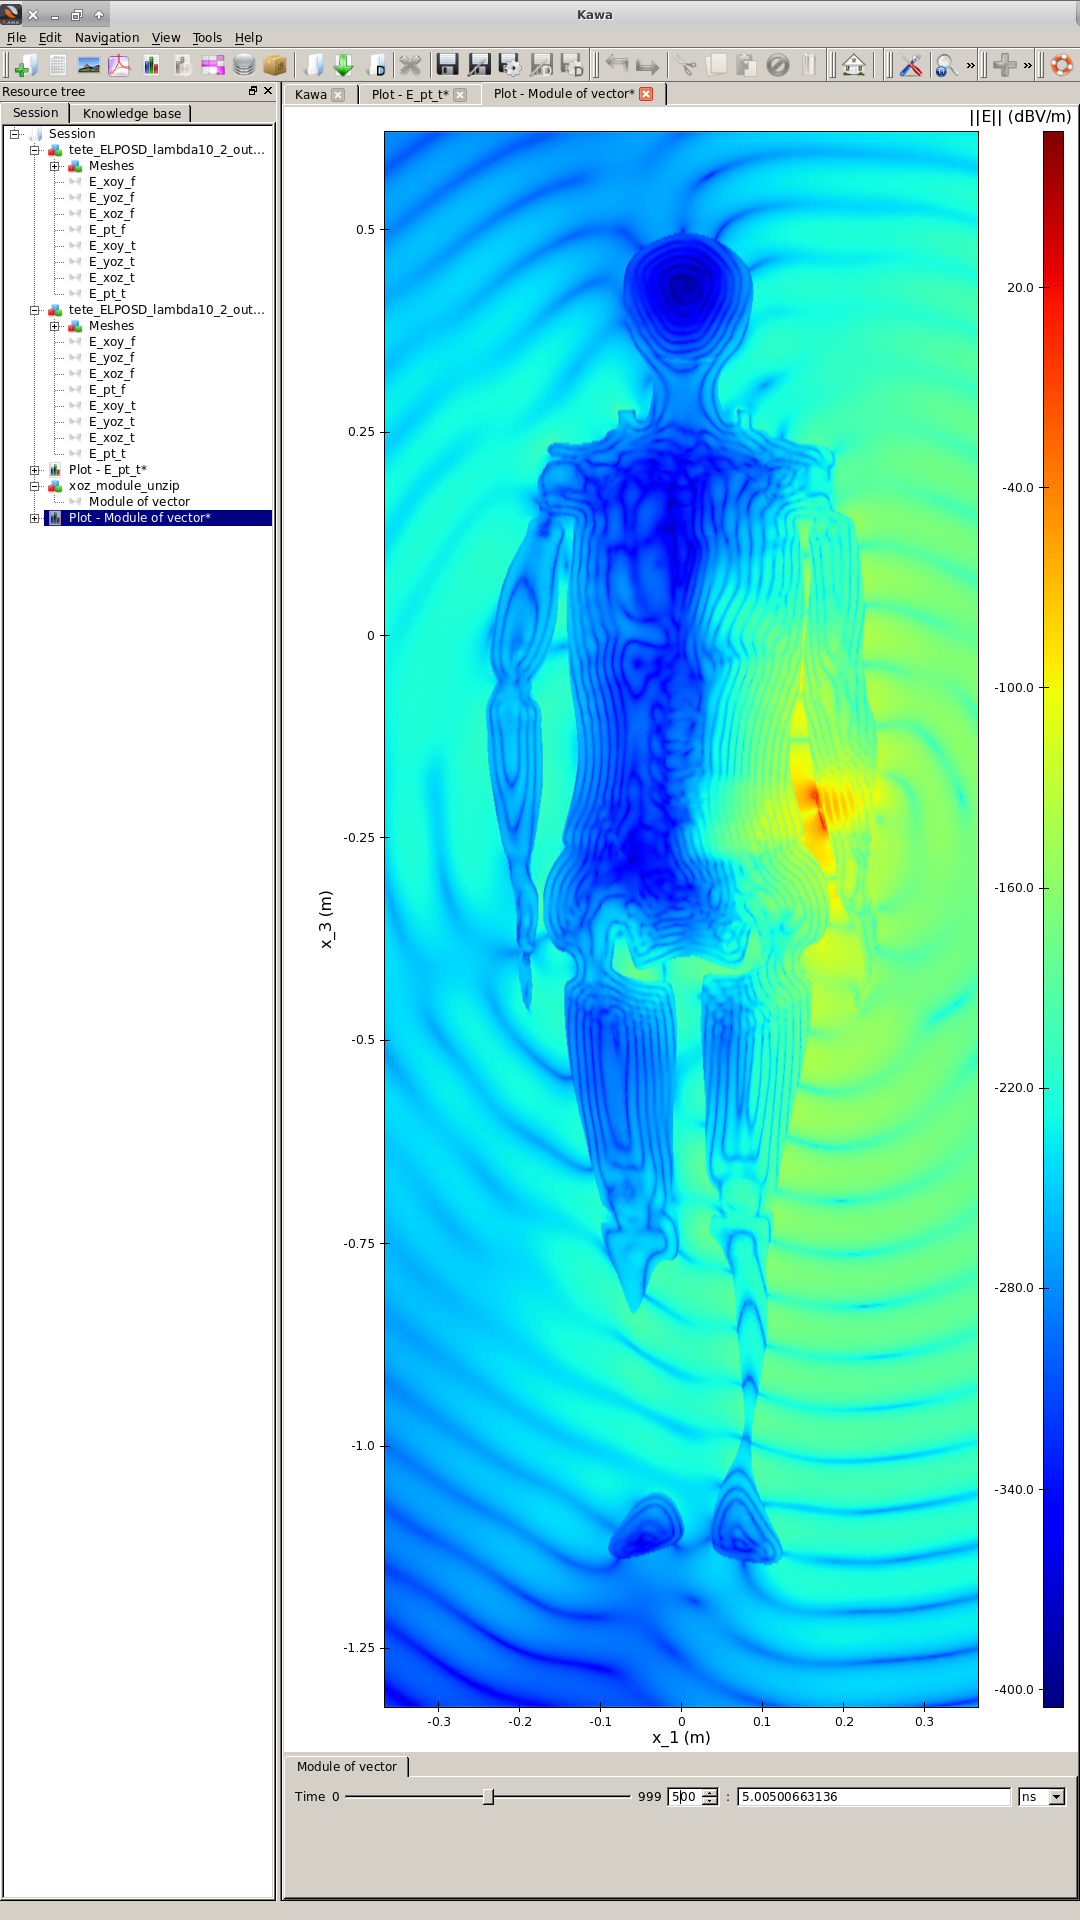
\includegraphics[
	width=0.66\linewidth,
	trim={317 170 8 108},clip
	]{kyoto_5ns}
\end{figure}

\begin{figure}[!h]
	\centering
	\caption{
		\label{img:annexe_kyoto_cutplane_6ns}
		Résultats en plan de coupe $(\x_1 O \x_3)$
		en $\x_2 = -0.1255$ m (antenne)
		au temps $t=6$ ns.
	}
	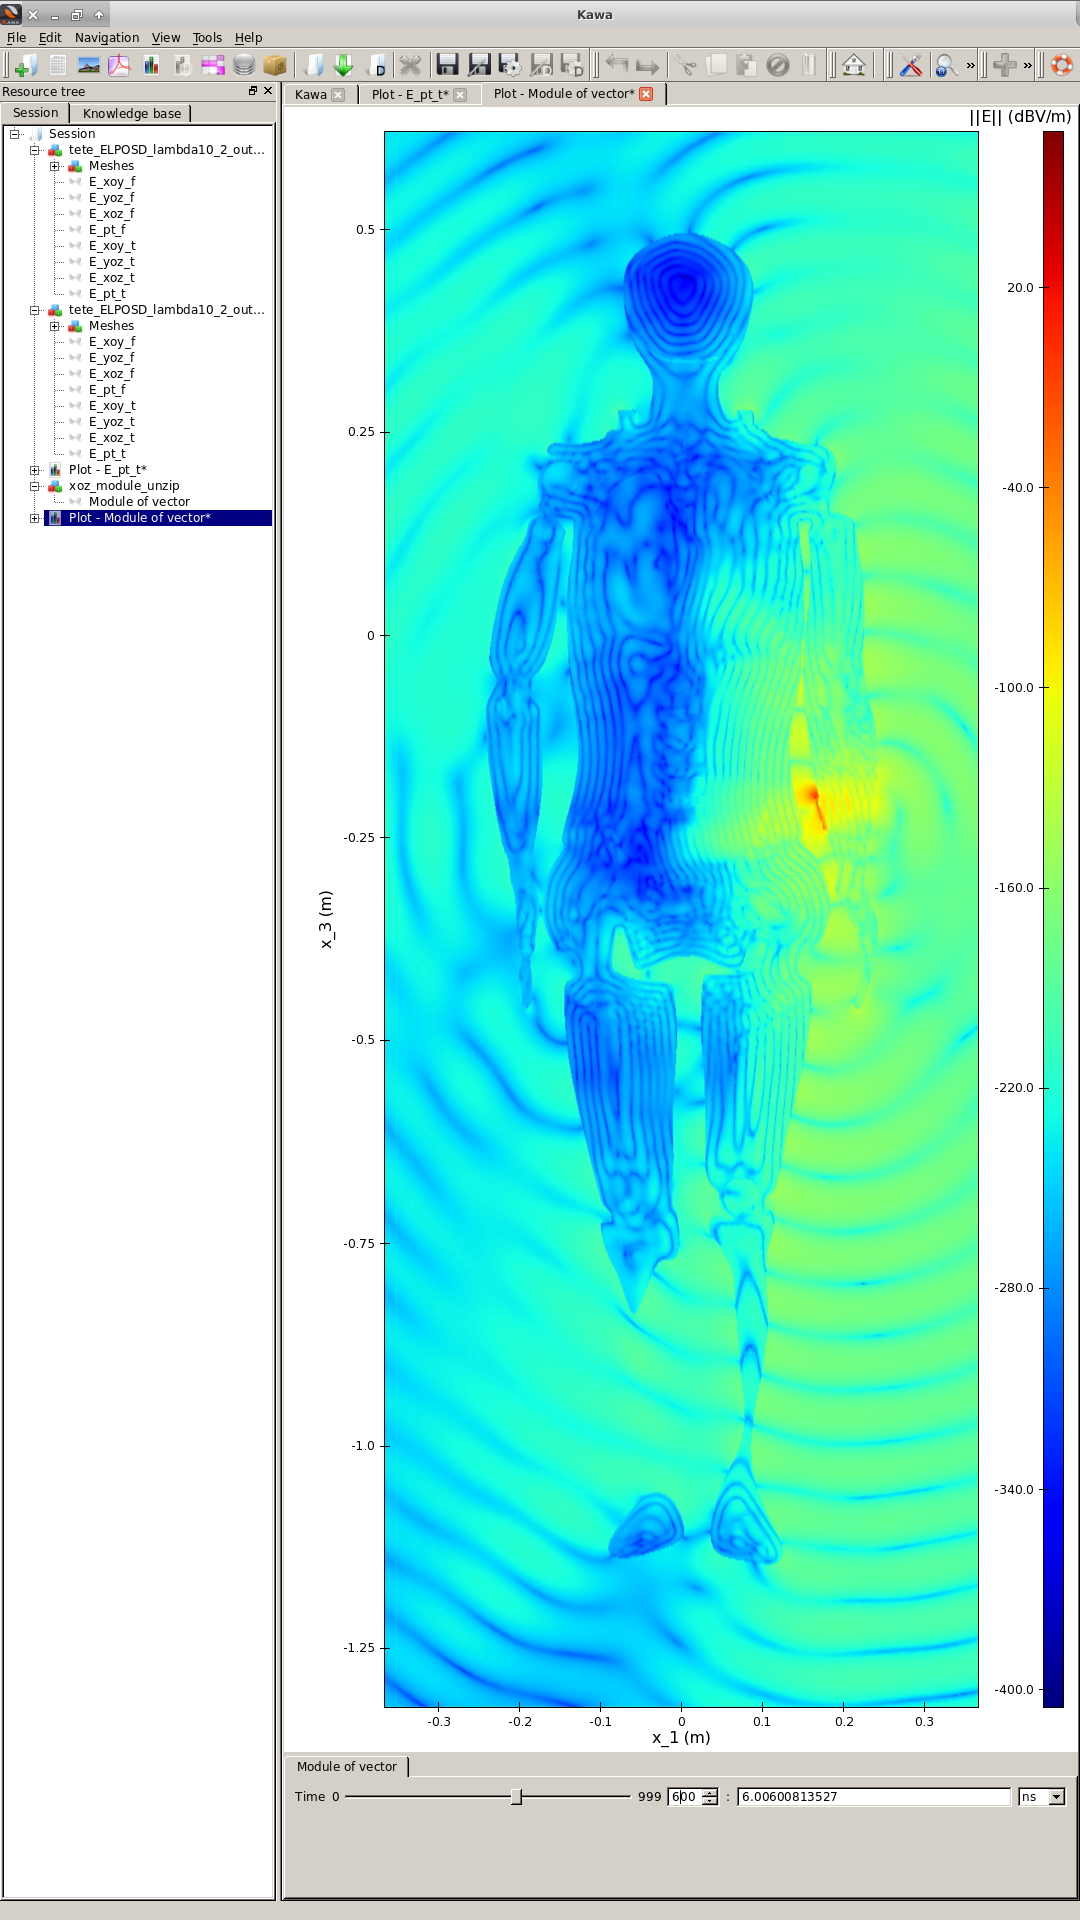
\includegraphics[
	width=0.66\linewidth,
	trim={317 170 8 108},clip
	]{kyoto_6ns}
\end{figure}

\begin{figure}[!h]
	\centering
	\caption{
		\label{img:annexe_kyoto_cutplane_7ns}
		Résultats en plan de coupe $(\x_1 O \x_3)$
		en $\x_2 = -0.1255$ m (antenne)
		au temps $t=7$ ns.
	}
	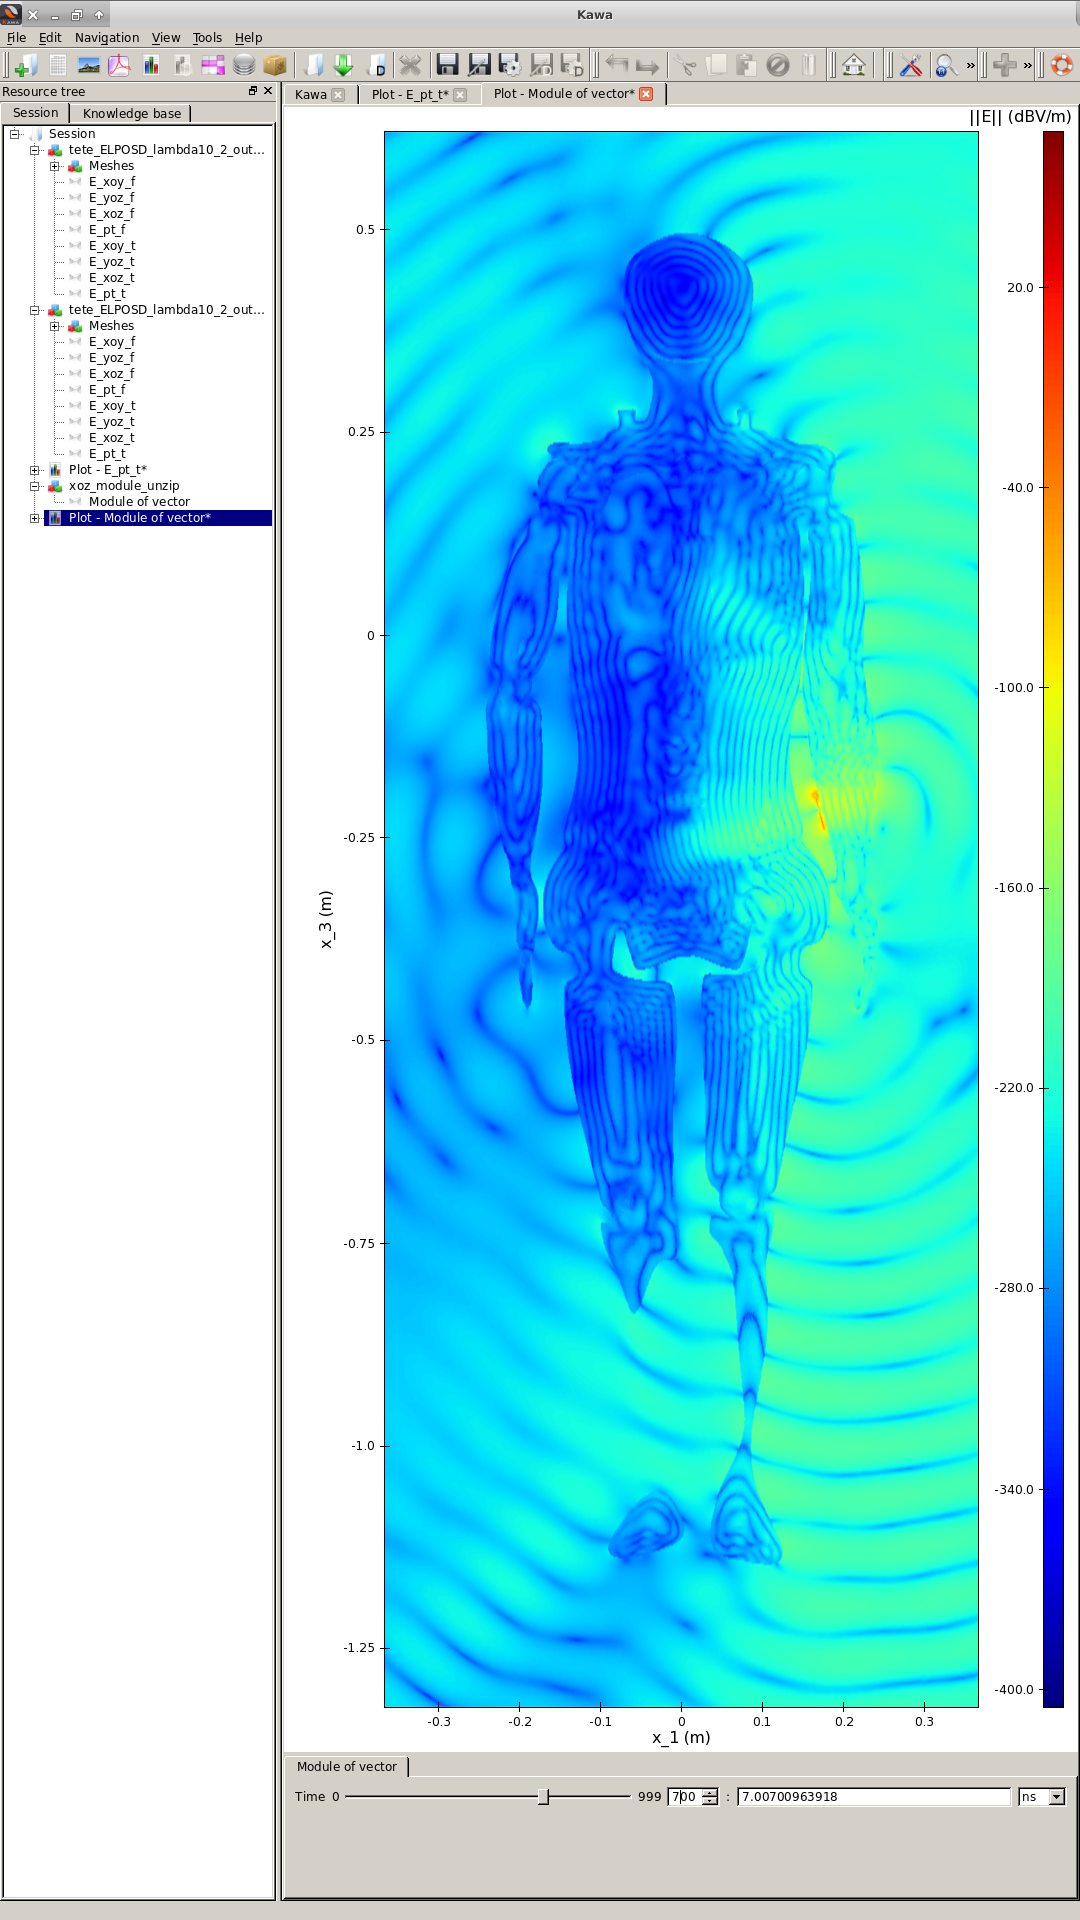
\includegraphics[
	width=0.66\linewidth,
	trim={317 170 8 108},clip
	]{kyoto_7ns}
\end{figure}

\begin{figure}[!h]
	\centering
	\caption{
		\label{img:annexe_kyoto_cutplane_8ns}
		Résultats en plan de coupe $(\x_1 O \x_3)$
		en $\x_2 = -0.1255$ m (antenne)
		au temps $t=8$ ns.
	}
	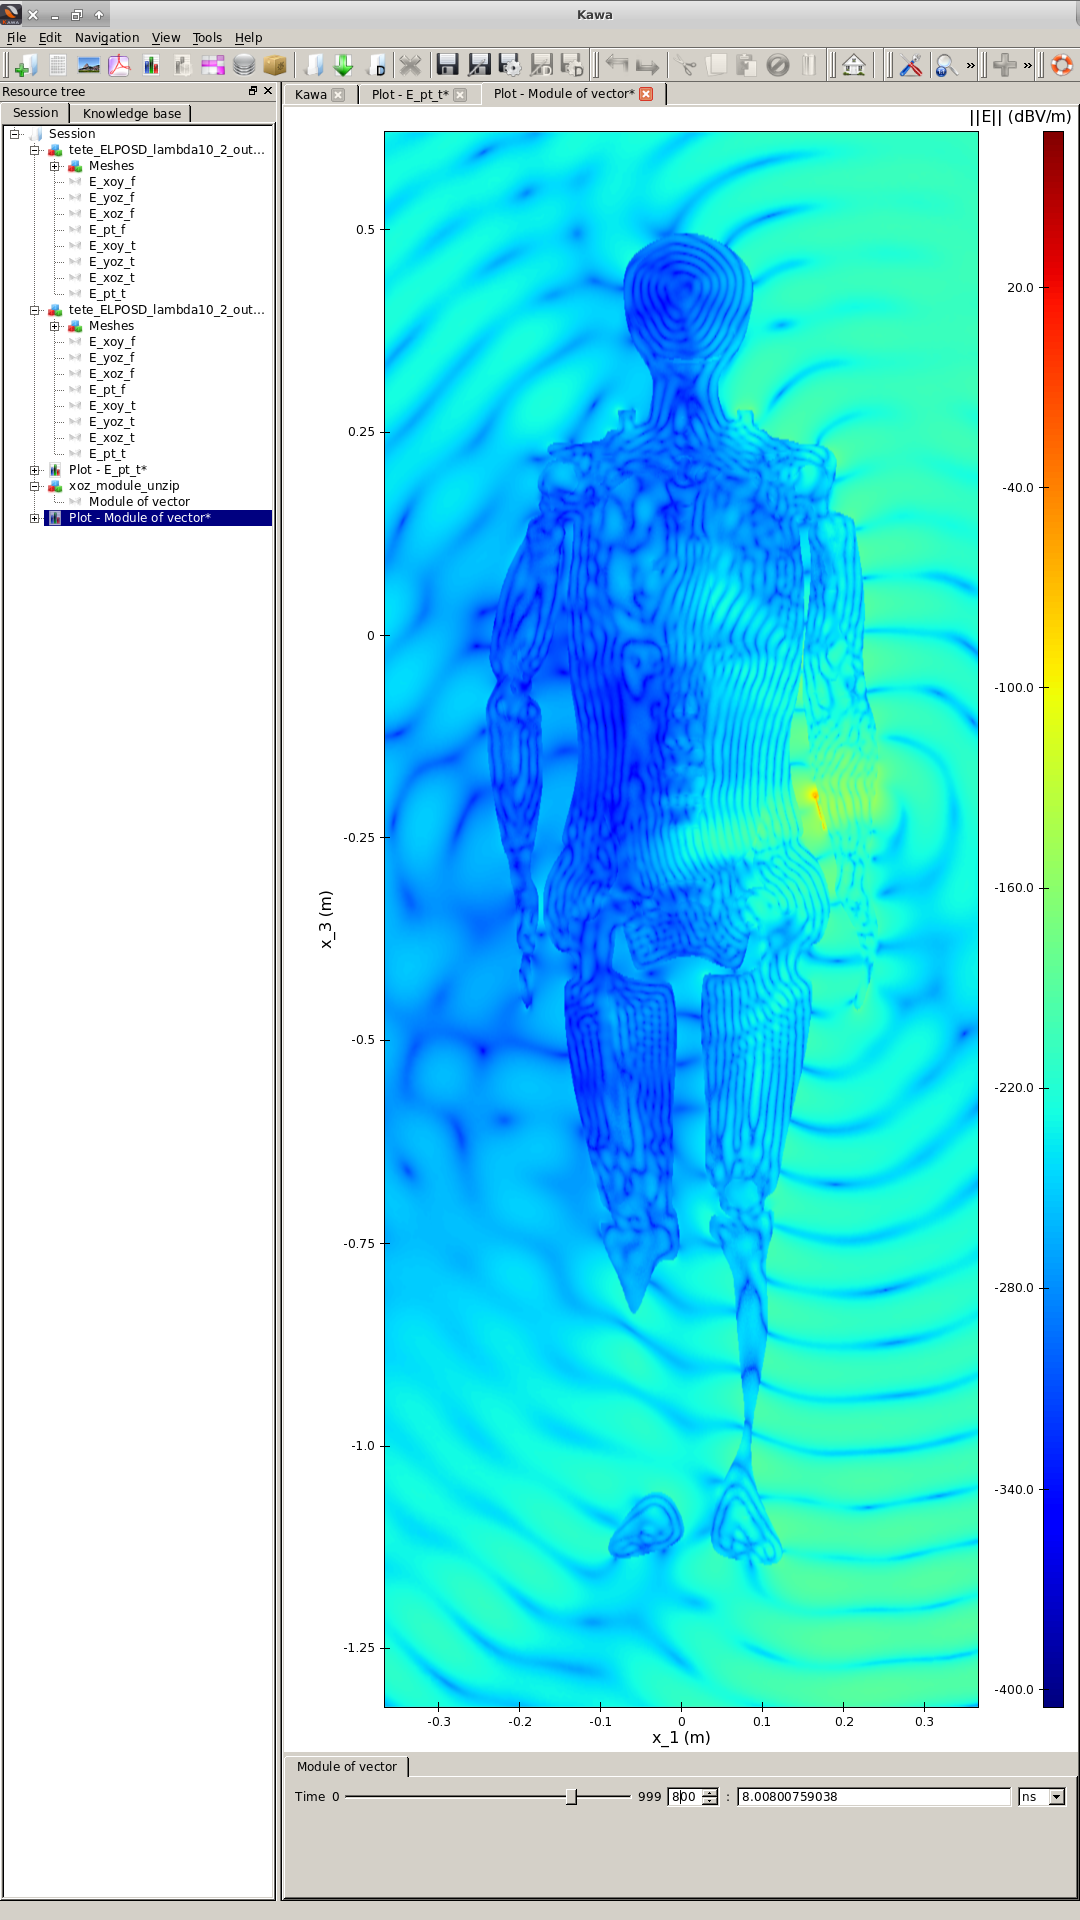
\includegraphics[
	width=0.66\linewidth,
	trim={317 170 8 108},clip
	]{kyoto_8ns}
\end{figure}

\begin{figure}[!h]
	\centering
	\caption{
		\label{img:annexe_kyoto_cutplane_9ns}
		Résultats en plan de coupe $(\x_1 O \x_3)$
		en $\x_2 = -0.1255$ m (antenne)
		au temps $t=9$ ns.
	}
	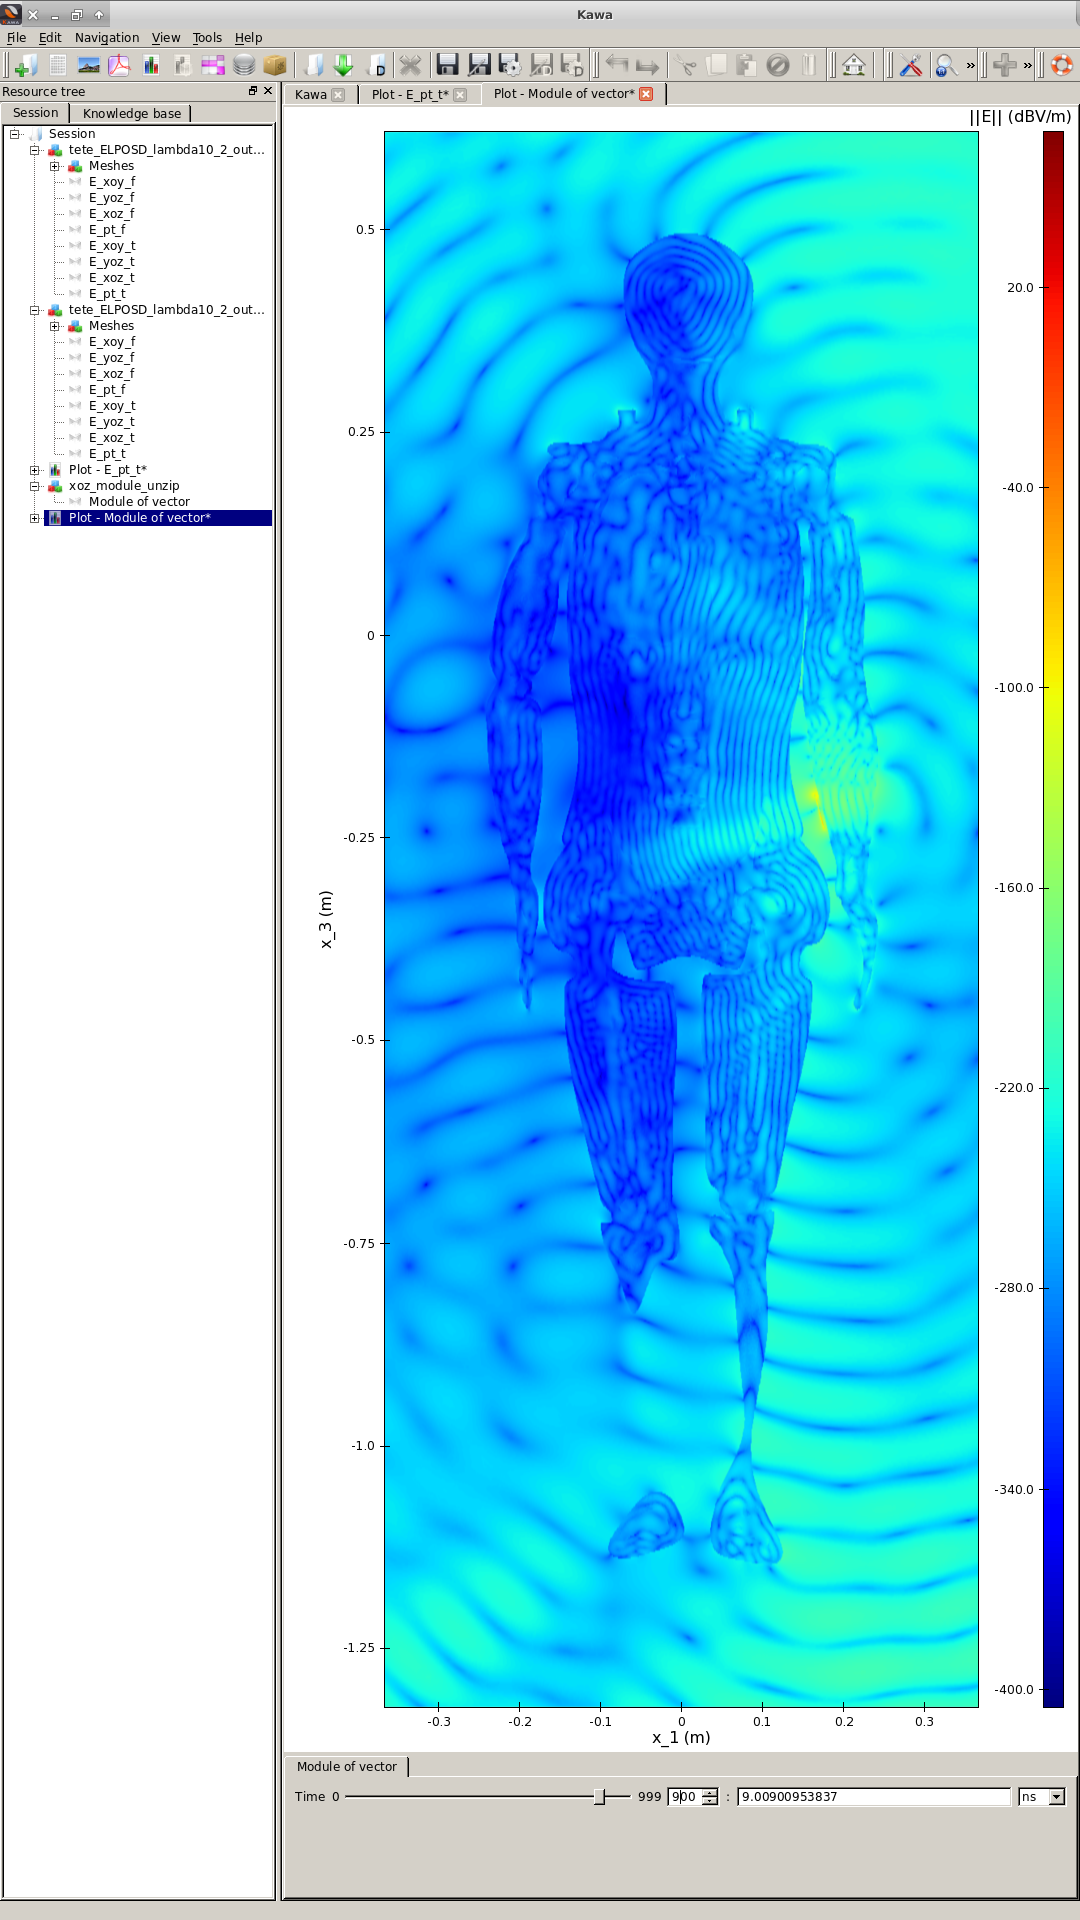
\includegraphics[
	width=0.66\linewidth,
	trim={317 170 8 108},clip
	]{kyoto_9ns}
\end{figure}

\begin{figure}[!h]
	\centering
	\caption{
		\label{img:annexe_kyoto_cutplane_10ns}
		Résultats en plan de coupe $(\x_1 O \x_3)$
		en $\x_2 = -0.1255$ m (antenne)
		au temps $t=10$ ns.
	}
	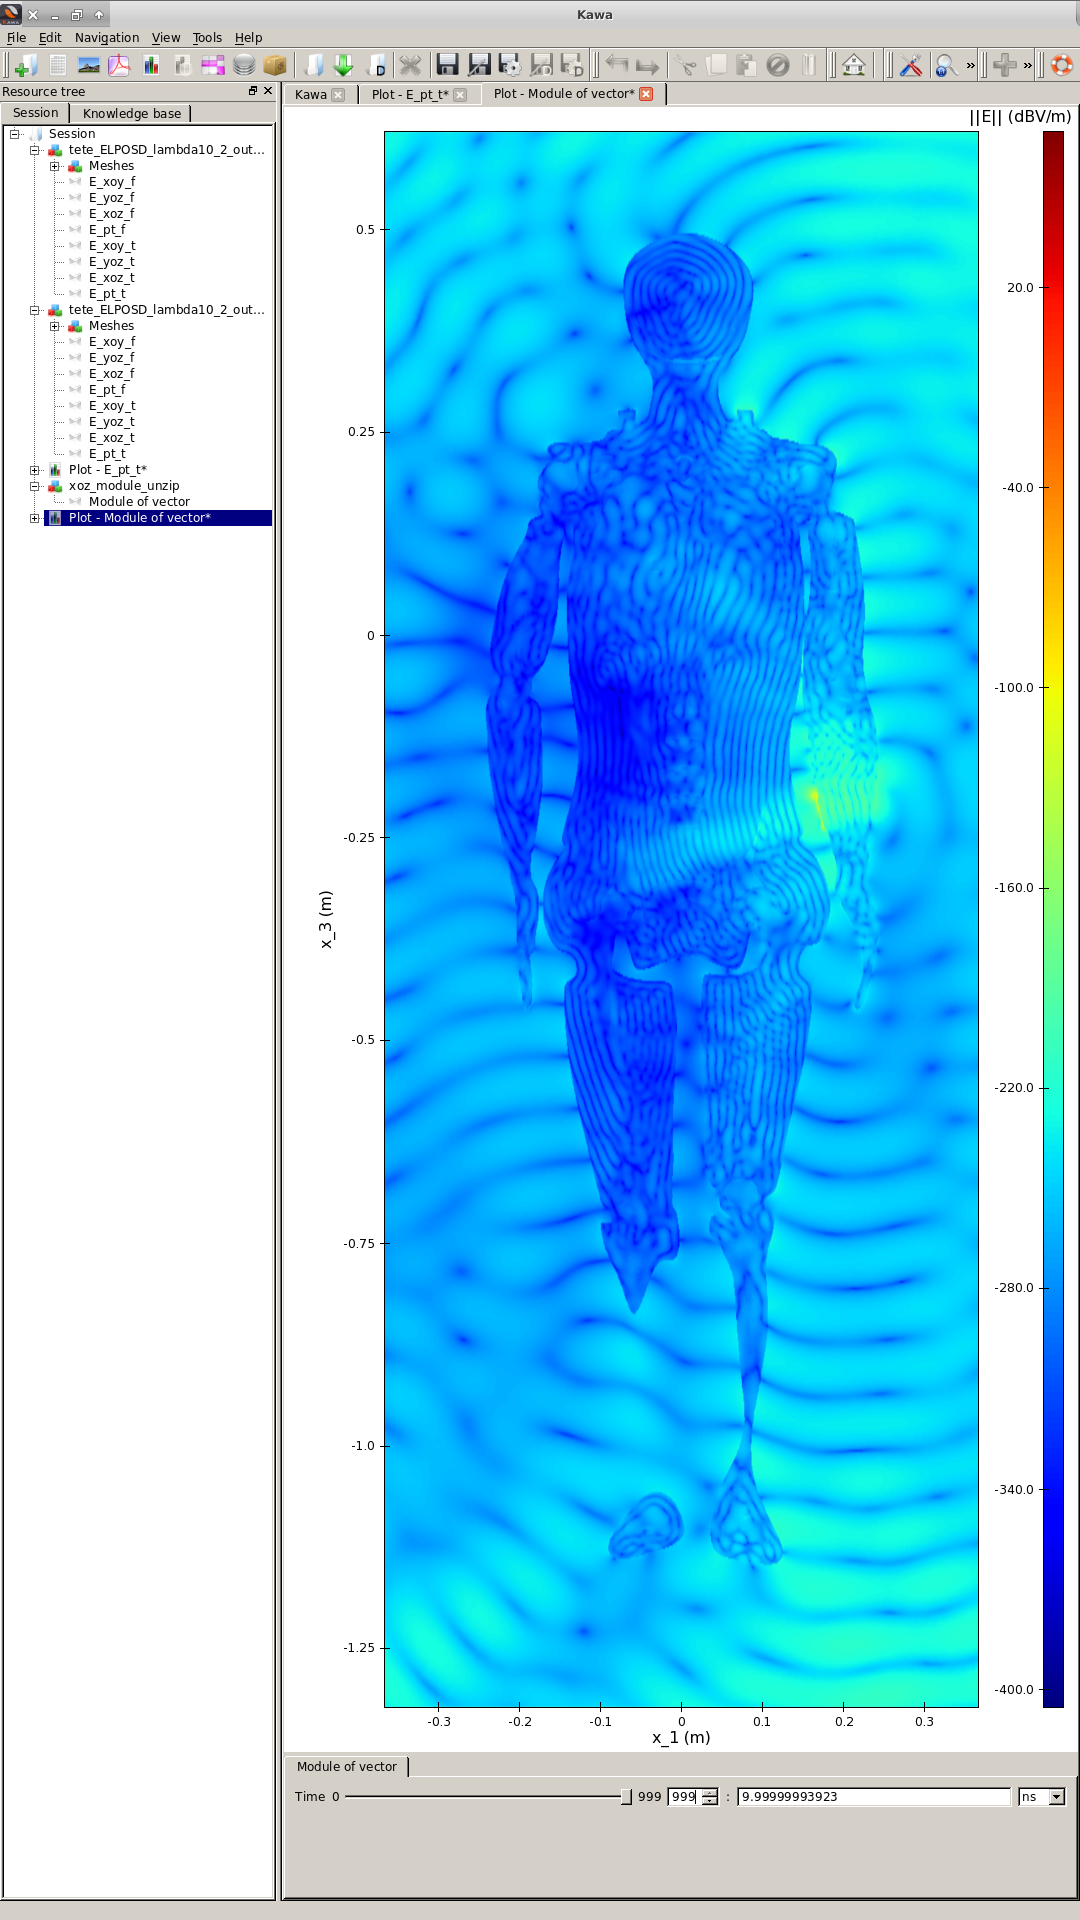
\includegraphics[
	width=0.66\linewidth,
	trim={317 170 8 108},clip
	]{kyoto_10ns}
\end{figure}

